% $Id: solution.tex 1784 2012-04-27 23:29:31Z nicolas.cardozo $
% !TEX root = main.tex

\chapter{Solution}
\label{cha:solution}

As mentioned earlier, the black box problem is not new, and it is something 
that can be addressed using a debugger. However, currently, there is no 
debugger capable of working with RL programs. The reason for this is that 
most of the debuggers are postmortem, or they don't allow you to go back in 
time. Also, most of the debuggers don't allow you to modify variables, and in 
order to improve and debug \ac{RL} programs we should be able to perform 
specifically the following features:

\begin{itemize}
    \item Stepping back: due to the execution cycle of an \ac{RL} program we 
    want to have a functionality that will allow us to step back and change 
    the value of a variable. This will allow us to check if the problem is a 
    not well design hyperparameter, or it will let us interact directly with 
    the code without stopping the execution and losing the state of the program 
    and the time training.
    \item Modifying variables: just as we said before, we would want to have a 
    tool that will let us modify the variables during execution time. Which means
    that the tool must not kill the program, but keep working with the state, 
    and variables.
\end{itemize}

Therefore, the proposed solution in this work is the creation of a debugger with the 
functionalities mentioned above, as they provide more value to debug \ac{RL} agents. This 
is not a traditional debugger; rather, it allows for an understanding of the 
internal state of the agent, the decisions it makes, and the rewards it 
receives. In other words, it allows the developer to interact with the program, modify
variables, and continue the program's execution, by allowing to understand 
the execution context of the agent in terms of variables, environment, and rewards. 

Additionally, aims to provide a deeper understanding of the behavior of 
RL programs and to identify errors that arise during the learning process. 
This would allow for the evaluation of the construction and quality of 
software developed for RL and help formulate strategies to improve the 
development of these programs.

Thus, this solution proposes a framework that enables developers to 
analyze RL programs, evaluate their behavior, and observe the evolution 
of different variables over time.

In this chapter, we present the design and implementation of the debugger tool: \ac{Flik}.
The debugger is a key component of the proposed framework, as it allows 
developers to interact with the RL program during execution, inspect the 
internal state of the agent, and modify its behavior in real-time.

\ac{Flik} is a console-based debugger, based on \ac{PDB} debugger. Add features 
such as colored syntax highlighting, tracking of variable states, and capturing stdout output 
from executed lines. The following are the three major features \ac{Flik} has:
\begin{itemize}
    \item \ac{Flik} saves the state in each step, it saves the local and global variables, 
    in a history variable. Additionally, other metadata like the information of the line 
    being executed is saved. This allows us to work later on the stepping back feature.
    \item Additionally, \ac{Flik} knows how to restore a previous state of a program, as 
    in the previous feature saves every information needed from the stack and the variables 
    to restore the state based on the history.
    \item Finally, \ac{Flik} performs the stepping back feature, it is created as a custom 
    \ac{PDB} command, and it has the same format as any other command. This takes the state
    saved in the specific line of code you want to step back, and it restores the state according
    to that information.
\end{itemize}

In Python, the internal state during execution is primarily encapsulated in 
stack frames. Each stack frame contains information about the execution state of a function 
call, including the current line number, local and global variables, and other metadata:
\begin{itemize}
    \item $f\_lineno$: The current line number being executed.
    \item $f\_locals$: A dictionary of local variables within the frame.
    \item $f\_globals$: A dictionary of global variables accessible within the frame.
    \item $f\_code$: A code object representing the function's bytecode and source code metadata.
\end{itemize}
The state is saved in a list that stores snapshots of the frame's state (line and variables) 
at each step, which allows stepping back the state being restored. The exec function can execute 
in a list that stores snapshots of the frame's state (line and locals) at each stepcode in a 
specified frame's context by passing $f\_globals$ and $f\_locals$ as parameters. This allows 
\ac{Flik} to simulate running a specific line in the context of a previous frame, maintaining 
both local and global variable references, essentially restoring the saved execution state.

This all done by extending the PDB class and adding custom commands to support stepping back
and a custom interface which allows the user to interact with the debugger. The interface 
displays the code, variables, and execution point, and allows the user (to use the \ac{PDB} 
functions) to pause, step forward, step back, continue or restart the program, as well as 
modify and inspect variables. 

\fref{fig:debuggerf} presents the general interface of \ac{Flik}, 
the upper frame is shown the execution running, in this case the print 
for the array to be sort. The middle frame shows the source code that is being 
debugged, the lower frame shows the variables that are being used in the 
program so far. Finally, in the lower part is the interactive console in which the user can 
send the corresponding commands to the debugger.

\begin{figure}[h]
    \centering
    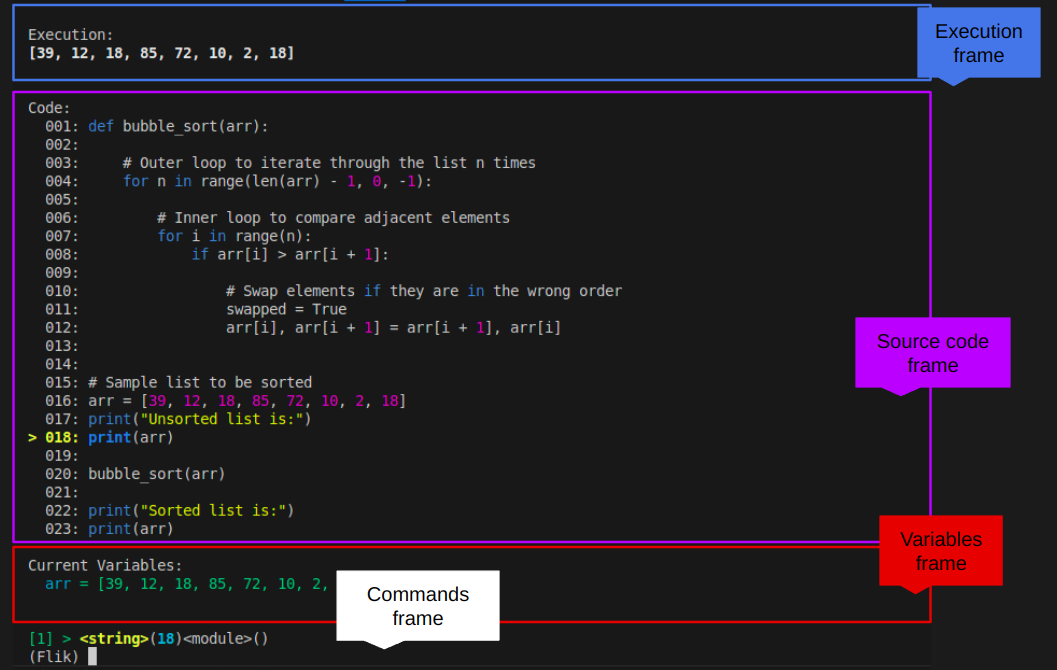
\includegraphics[width=1\textwidth]{figures/flik_interface.png}
    \caption{Debugger tool}
    \label{fig:debuggerf}
\end{figure}

% Add example of use step by step. Explain the videos.
Now, let's use an example to further understand how \ac{Flik} works. Let's work with 
the usual gridworld example of \ac{RL} programs. The environment is a grid of 
$10 \times 10$ and the agent can move in four directions: up, down, left, and right.
There are two kind of rewards that the agent can get, a positive reward of 1 when 
the agent gets to the goal, and a negative reward of -1 when the agent goes to the 
trap. The agent starts in the blue box shown \fref{fig:gridworld}. Now, in the following
example let's say we define our program properly, but we define the $\epsilon$ value 
so small that the agent will not explore the grid, and will not learn properly. 
This will mean that only the first action taken by the agent will be random and after that
with a major probability it will keep only choosing the same action. We can think about 
the worst case scenario, in which the agent will move right and then in the next step it 
will move left, and it will keep doing this for a long time, with a low probability of 
choosing another action. We can use \ac{Flik} to debug this problem, we can go step by step
inspecting the variables and the actions taken and we can identify specifically that for 
the first state in each episode the agent is taking the same action. We can then go back and
reproduce this problem as many times as we want, and we can change the value of $\epsilon$
to a higher value, so the agent can explore the grid properly. And finish the execution.
This example is shown in the following video: \url{https://drive.google.com/file/d/1NyipuWsRr6ZrIbtlvU5qyooHS2aVsWXc/view?usp=sharing}.



\endinput

